%%%%%%%%%%%%%%%%%%%%%%%%%%%%%%%%%%%%%%%%%%%%%%%%%%%%%%%%%%%%%%%%%%%%%%%%%%%%%%%%%%%%%%%%%%%%%%%%%%%%%%%%%%%%%%%%%%%%%%%%%%%%%%%%%%%%%%%%%%%%%%%%%%%%%%%%%%%%%%%%%%%%%%%%%%%%%%%%%%%%%%%%%%%%
% Written By Michael Brodskiy
% Class: International Relations
% Professor: J. Kropf
%%%%%%%%%%%%%%%%%%%%%%%%%%%%%%%%%%%%%%%%%%%%%%%%%%%%%%%%%%%%%%%%%%%%%%%%%%%%%%%%%%%%%%%%%%%%%%%%%%%%%%%%%%%%%%%%%%%%%%%%%%%%%%%%%%%%%%%%%%%%%%%%%%%%%%%%%%%%%%%%%%%%%%%%%%%%%%%%%%%%%%%%%%%%

\documentclass[12pt]{article} 
\usepackage{alphalph}
\usepackage[utf8]{inputenc}
\usepackage[russian,english]{babel}
\usepackage{titling}
\usepackage{amsmath}
\usepackage{graphicx}
\usepackage{wrapfig}
\usepackage{enumitem}
\usepackage{amssymb}
\usepackage[super]{nth}
\usepackage{everysel}
\usepackage{ragged2e}
\usepackage{geometry}
\usepackage{fancyhdr}
\usepackage{cancel}
\usepackage{siunitx}
\usepackage{xcolor}
\usepackage{setspace}
\usepackage{censor}
\doublespacing
\geometry{top=1.0in,bottom=1.0in,left=1.0in,right=1.0in}
\newcommand{\subtitle}[1]{%
  \posttitle{%
    \par\end{center}
    \begin{center}\large#1\end{center}
    \vskip0.5em}%

}
\pagestyle{fancy}
\fancyhf{}
\fancyheadoffset{0cm}
\renewcommand{\headrulewidth}{0pt} 
\renewcommand{\footrulewidth}{0pt}
\fancyhead[R]{\thepage}
\fancypagestyle{plain}{%
  \fancyhf{}%
  \fancyhead[R]{\thepage}%
}
\renewcommand{\headrulewidth}{0pt}
\usepackage{hyperref}
\hypersetup{
colorlinks=true,
linkcolor=blue,
filecolor=magenta,      
urlcolor=blue,
citecolor=blue,
}

\urlstyle{same}


\date{}
\author{\normalsize \textbf{The Coming War With China}\\\normalsize  \censor{\textsc{Michael D. Brodskiy}}\\\normalsize  Department of Political Science, Diablo Valley College\\\normalsize  POLSC-250: International Relations\\\normalsize  Professor Kropf\\\normalsize  July 22, 2021}

% Mathematical Operations:

% Sum: $$\sum_{n=a}^{b} f(x) $$
% Integral: $$\int_{lower}^{upper} f(x) dx$$
% Limit: $$\lim_{x\to\infty} f(x)$$

\begin{document}

\maketitle

\newpage

\begin{abstract}
  \hspace{-17.5pt}This text is concerned with examining the coming war between the United States, a thalassocracy, and the People's Republic of China, the chiefest Eurasian tellurocracy, and the origins of this geopolitical conflict and whether or not this conflict will escalate to belligerence. For your consideration, the following analysis will begin with an explanation of the underlining history of the United States foreign service apparatus and the contemporary role of the People's Republic of China with respect to the interests of the United States in a post-Soviet world. Once a realist geopolitical perspective has been established this text will attempt to compute a correlation of forces and means to determine the outcome of symmetric military engagement between the United States and the People's Republic of China. 
\end{abstract}

\emph{Keywords}: \textit{thalassocracy}, \textit{tellurocracy}, \textit{geopolitics}, \textit{realism}, \textit{correlation of forces}

\newpage

\tableofcontents
\listoffigures

\newpage

\begin{center}
\section{\normalsize The Coming War With China}
\end{center}

\begin{center}
\subsection{\normalsize Geopolitics and the Realist Perspective}
\end{center}
\paragraph{Realpolitik} Geopolitics is the nomenclature designated for the pseudoscientific discipline at the crossroads of international relations, geography, and history. It is the tool with which foreign policy is crafted. Since its conception as the driving theory behind Anglo-Saxon sea power (See Alfred T. Mahan's \emph{The Influence of Sea Power Upon History: 1660–1783} (1890).) and the corresponding resistance to Eurasian transcontinental hegemony (i.e. Russian Empire, Union of Soviet Socialist Republics, People's Republic of China, etc.) it has been at the core of realpolitik (i.e.\ geopolitical realism) — the domineering geopolitical ideology of western, liberally democratic nation-states.
\paragraph{Era of Humiliation} When Mao Zedong and the communists defeated the nationalists during the Chinese revolutionary war he was able to utilize his political and socioeconomic doctrines to transform the land of his birth into the nation-state it is today. The founding of the People's Republic of China led to the utterance of the phrase “the end of the century of humiliation” — an idea largely championed by both the communists and the Kuomintang. The significance of that oration lies in the essence of that idea still being relevant at the epitome of Chinese foreign policy. Accompanying the triumphs of a classist Marxist-Leninist revolution, Zedong directed his statecraft at the ambition of eventually becoming a global hegemony. Although Mao Zedong has been deceased for almost half a century his followers in the Communist Party of China continue to aggressively carry out their mission of challenging the United States as the chiefest global hegemon. 
\paragraph{} In order to fully fathom the scope of the coming war with China, it is of the utmost importance to commence the geopolitical analysis at the period succeeding the Second World War, when Chinese communists did not yet control the governing regime and the United States foreign service apparatus was still in its infancy.
\begin{center}
\subsection{Heartland vs. Rimland}
\end{center}

\begin{wrapfigure}{R}{0.7\textwidth}
\centering
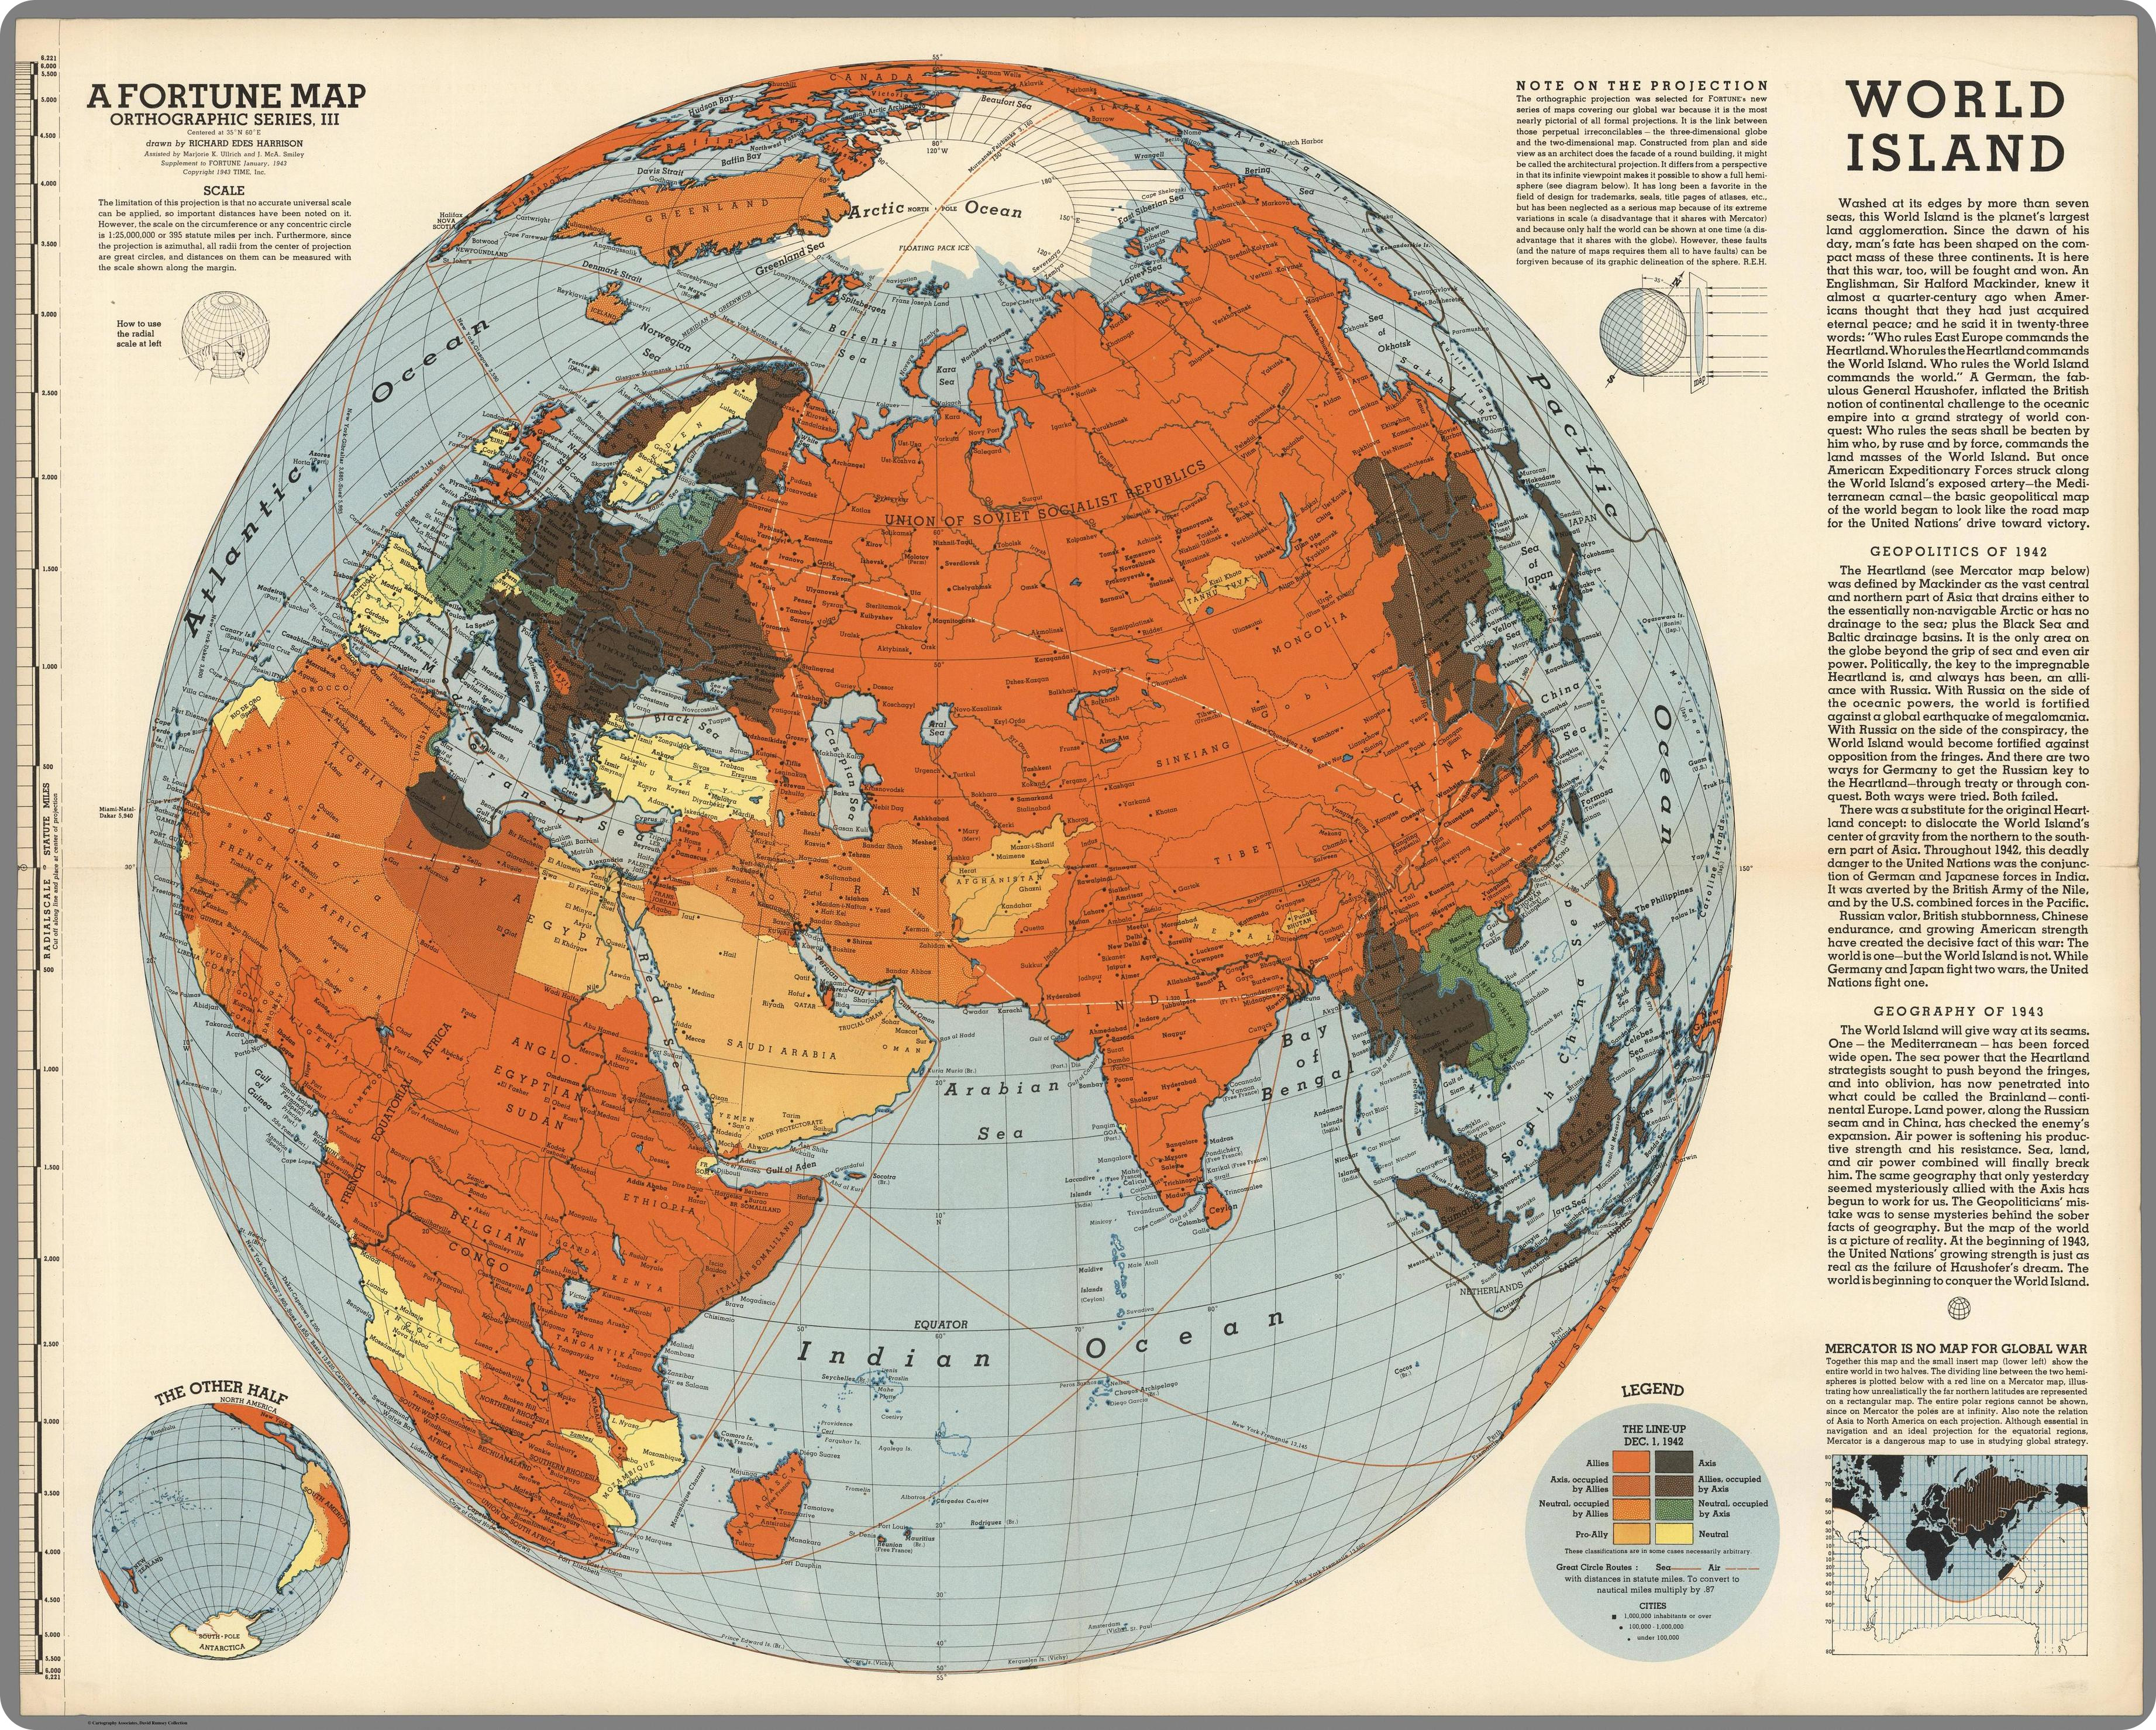
\includegraphics[width=0.65\textwidth]{Images/World_Island.jpg}
\caption{Map showing the World Island (\footnotesize{\emph{published by Fortune Magazine in} 1943})}
\label{fig:fig1} 
\end{wrapfigure}
%\begin{figure}[h!]
  %\centering
  %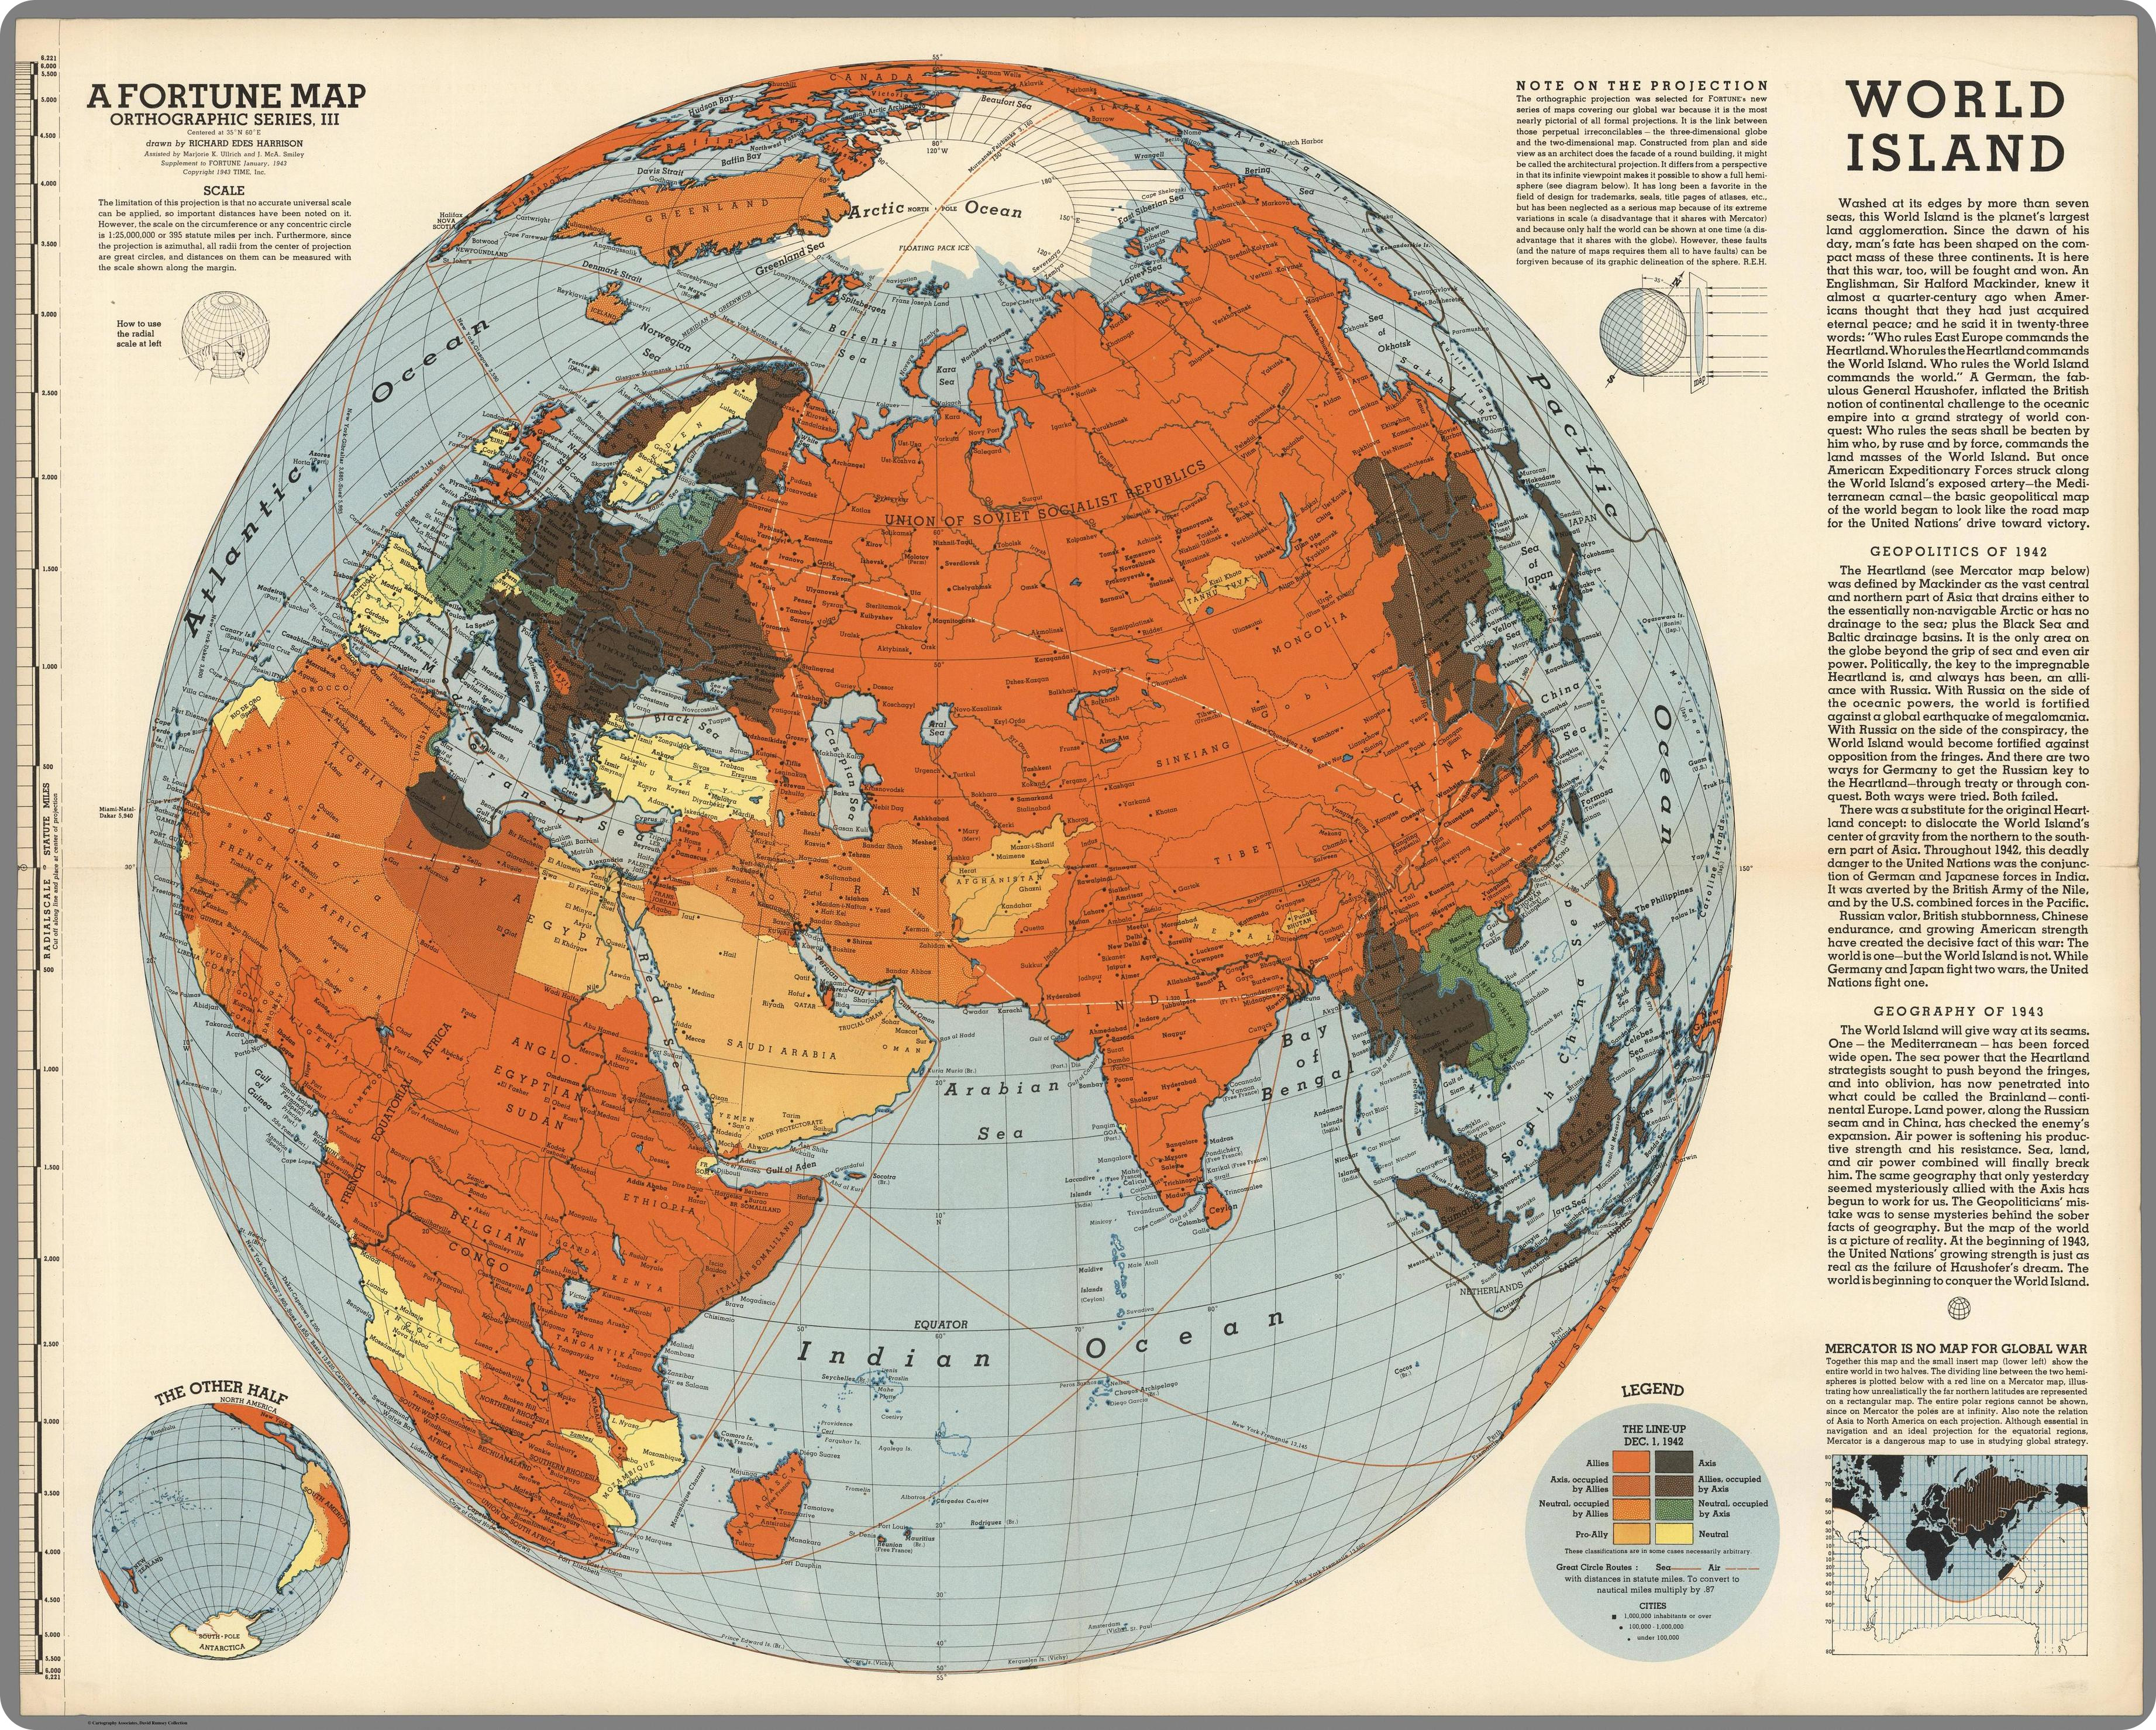
\includegraphics[width=\textwidth]{Images/World_Island.jpg}
  %\caption{\small{Map showing the World Island (\emph{published by Fortune Magazine in} 1943)}}
  %\label{fig:1}
%\end{figure}

\paragraph{A Thalassocratic Hegemony} Almost one-hundred years ago, the United States triumphed in tandem with the Soviet Union over the annihilated Third Reich. In addition to the prosperity of peacetime, this triumph signified a new geopolitical epoch of ideological polarization. A polarized globe, separated by boundaries primarily attributable to geographical phenomena, beyond the control of human narcissism, became the inevitable arena of contest. Divided by mountains, plains, and seas with inaccessible coastlines, a new convention (refer to \textbf{Figure \ref{fig:fig1}}) assumed an integral role in geopolitical discourse. Land power vs sea power — otherwise referred to as the “Heartland vs Rimland theory” (Spykman, 1944). The preceding convention, in accordance with Halford Mackinder's thesis of his most recognizable literary work, \emph{Democratic Ideals and Reality}, “[w]ho rules Eastern Europe commands the Heartland. Who rules the Heartland commands the World Island (The World Island — Europe, Asia, and Africa). Who rules the World Island commands the world,” (Mackinder, 1919) was the underlining premise for the Third Reich's reciprocation of the Brusilov Offensive (Russian general Aleksey Brusilov's coordinated three pronged northern, central, and southern advance against German and Austrian-Hungarian armies of the Eastern Front in World War One.) under the pretense of a preemptive invasion. The largest land oriented military endeavor in the history of warfare, Operation Barbarossa, designed to force Moscow to capitulate, inadvertently caused the eventual Soviet pincering of all three German kampfgruppen (army formations) and subsequent push back to and occupation of Berlin. World domination and, peripherally, the accumulation of lebensraum (popularized colonial resettling) was believed to be impossible without conquering the Russian landmass (i.e.\ heartland). Justified by the Third Reich's antipathy toward Marxism-Leninism, Operation Barbarossa was speculated to conquer the World Island, and, as prophesized by Mackinder, the world. Although unsuccessful, the Second World War forced western geopoliticians to reconsider the shortcoming of Mackinder's thesis. As aforementioned, the new geopolitical epoch of ideological polarization following the emergence of the United States and Soviet Union as undisputed superpowers took the form of a thalassocratic vs tellurocratic struggle, evident by the American continent's independence from the World Island (i.e. Atlantic and Pacific oceans). In essence, the same principle which left the United States mainland unscathed during World War Two was responsible for formulating the United States diplomatic mission for years to come. Gone were the days of total war fanaticism; the miscalculations of the western, with respect to Russia, invaders (i.e.\ Hitler's and Napoleon's armies), would become distant memories with the reposturing of the United States after World War Two. Russia, or rather the RSFSR and, by extension, the entirety of the Soviet Union, was surrounded by hostile to Marxism-Leninism nation-states, lacked significant warm water ports, and suffered from the vatsness of landlocked lines of communication (majority of which were severely crippled as a result of the German invasion). In this manner, Soviet foreign policy was dealt the weaker hand, accustomed to the dominant role of the tellurocratic hegemon, the United States materialization into a complementary thalassocratic hegemon was an unparalleled, assymmetric response to Soviet aggression throughout the heartland. Therefore, the new geopolitical epoch of ideological polarization set the stage for heartland nation-states (i.e.\ Socialist Bloc) against the rimland nation-states (i.e.\ Capitalist Bloc) with diplomats and intelligence officers actively operating on the front lines of a new, unconventional global amphitheater.
\begin{center}
  \section{\normalsize Geopolitical Future of the United States}
\end{center}
\begin{center}
\subsection{\normalsize American Resourcefulness vs. Marxist-Leninist Anti-Deviationism}
\end{center}
\paragraph{The American Diplomatic Mission} It should come as no surprise that the diplomatic rhetoric surrounding American foreign relationships after the Second World War was rooted in the same nomenclature associated with the thalassocratic nature of the United States (i.e.\ North \underline{Atlantic} Treaty Organization, \underline{Naval} Information Warfare Center, \underline{Atlantic}/\underline{Naval} Information Warfare Systems Command, \underline{Navy} Field Operational Intelligence Office, etc.). The oldest member organizations of the intelligence community were naval intelligence directorates which received a post World War increase in congressional funding to aid in signals intelligence gathering against their Soviet Naval counterparts. The enactment of commerce treatises among rimland nation-states and the sanctioning of pro-Soviet heartland states, considered in tandem with the formation of militaristic partnerships, such as the aforementioned NATO, is a direct manifestation of the geopolitical struggle between Soviet Union and the United States, heartland vs rimland, respectively. The inclusion of rimland nation-states into NATO only strengthens the assertion that the United States predominant long term diplomatic objective was to foster relationships with rimland nation-states to further \emph{landlock} the Soviet tellurocratic hegemony. Likewise the coup d'\'etats and ensuing conflicts in Guatemala, Iran, Malaysia, Vietnam, Cambodia, Angola, Mozambique, Greece, Nicaragua, and Afghanistan (Although Afghanistan is landlocked and therefore not a rimland state, it had the distinct characteristic of bordering the Soviet Union.) serve as prime examples of the effects of the anaconda theory in action. As described by Russian geopolitician Aleksandr Dugin, the cold war was a series of “\selectlanguage{russian}традиционного атлантистского плана по `удушению'  \dots [стратегия `кольца анаконды'] \dots континентальных просторов материка через захват прибрежных территорий по всей протяженности Евразии, и особенно на Юге и Западе.” \selectlanguage{english}(Dugin, Foundations of Geopolitics, 1997), which loosely translates to \emph{the traditional Atlantic plan of} `\emph{suffocating}' \dots [`\emph{anaconda ring}' \emph{strategy}] \dots \emph{the continental vastness of the heartland through the seizures of coastal territories throughout the length of Eurasia}, \emph{especially in the south and west}. Perhaps the term seizures is inappropriately used, as the United States carefully fostered diplomatic relationships with geopolitical partners belonging to NATO and OPEC in the aforementioned regions of influence. In any case, the anaconda containment maneuver utilized by the United States can effectively be recognized as a crucial geopolitical aspect of the Cold War. Consequently, the existence of both military and political institutions associated with strengthening the rimland partnerships of the United States demonstrate their genesis out of necessity, as opposed to ideological fanaticism. That is to say, the United States, fundamentally, does not need to justify any political course of action, to appease a particular political platform, actor, or party. The benefit of relying on senior diplomats and intelligence officers divorced from domestic political affiliations enables the United States to assume a realist perspective. Consider the inverse of this phenomena in a unilaterally politicized nation-state like the Republic of China or former Soviet Union; any action must be justified by Marxist-Leninist principles to ensure loyalty to the Central Executive Committee of the Chinese Communist Party. This unfortunately cripples a realist perspective and moreover detriments constructive diplomatic dialogue and any potential relations. In other words, a foreign service independent from institutionalized political indoctrination will always be able to operate clearer with a significantly more constructive realist discourse without regard for some pernicious party line. This is exactly why American resourcefulness was able to craft such strong partnerships, not only with Five Eyes (An intelligence alliance comprising of Anglo-speaking nation-states, and derivatives thereof.) allies, but also nation-states without shared commonality. International relations of such magnitudes would not even be conceivable by an oppressive Marxist-Leninism antideviationist regime. The ability to seek out transatlantic partnerships and practice corresponding diplomacy at the highest levels prepared the United States diplomats and intelligence officers for the post-Soviet geopolitical climate. Ater the disintegration of the Soviet Union a new tellurocratic hegemon was expected to emerge from the World Island, and while the People's Republic of China and Russia Federation collectively filled that void, they individually lack the necessary grandiosity; however, the former is rapidly growing its population, economy, and military capacity toward world conquest proportions and, while the United States, as a result of its rimland signature, maintains international relationships across the globe, the next major conflict, military or otherwise will be a result of Chinese expansion, or lack thereof.
\paragraph{Mainland China} As mentioned, the disintegration of the Soviet Union would not be possible without the active measures undertaken by American intelligence in tandem with the diplomatic strain imposed on the Socialist Bloc through various sanctions, coerced economic competitiveness, and `suffocation' of the heartland (i.e.\ anaconda strategy); and, while the result is the accumulation of years of painstakingly professional diplomatic and intelligence work, the United States is applying the same modus operandi toward the containment of Chinese aggression for a similar result in the pacific. Interestingly, the global amphitheater has not changed all that much since the days of the Soviet Union and United States bilaterally competing as heartland and rimland nation-states, respectively. An important premise however, is that unlike the Cold War post-World War Two epoch, the United States foreign service apparatus now has much more experience than any probable adversary in a thalassocratic/tellurocratic geopolitical struggle. With the Russian Federation existing as a mere fraction of the former might of the Russian Soviet Federative Socialist Republic, let alone the Soviet Union, in all aspects economical, military, and political, many geopoliticians exemplify the Republic of China's robustness in international markets as indication of their inevitable hegemony. While this may appear to be the case, it is in all actuality a rather specious conviction. Considering the case of China's rapid growth both intra- and internationally in conjunction with Schumpeterian convergence (\emph{catch}-\emph{up}) theory of macroeconomics, real GDP per capita across countries will eventually become equalized because poor countries will catch up to wealthy countries. What this implies is that the unprecedented increase in Chinese domestic technological industrialization is solely a characteristic of Chinese underdevelopment and not contrariwise. Any rejection of the empiricism accrued by the United States foreign service apparatus is detrimental to a proper analysis of the contemporary Chinese disposition. Currently, the predominant intelligence mission of the Chinese Ministry of State Security (\href{https://en.wikipedia.org/wiki/Ministry_of_State_Security_(China)}{MSS}.) is to play a bigger investor role in western Venture Capitalist endeavors (i.e. German think-tank researcher arrested on suspicion of spying for Chinese intelligence, Chinese state-linked cyber actor allegedly behind attack on global airline industry, China assesses emotions of subjects using AI technology that monitors skin pores, Belgian minister raises spy concerns about Chinese e-retail center at Liege airport, etc. (Fitsanakis, 2021)). Unlike the effectiveness of Russian SVR and GRU HUMINT officers, Chinese intelligence and security services are not as capable of penetrating western institutions through conventional espionage tradecraft, although there have been many attempted penetrations of the American intelligence community numerously in the past. In recognition of MSS shortcomings, Jia Chunwang (former Director of MSS and Procurator-general of the Supreme People's Procuratorate.), an alleged admirer of CIA, argued for the necessity in mimicking American intelligence as a result of his collaborations with his American counterparts during Operation Cyclone. In the interests of compensating for Chinese weaknesses in live source intelligence gathering and ability to successfully carry out both covert and clandestine operations, Chinese institutions indoctrinate from a maleable preadolsescent age that any tourist undertaking away from the mainland requires them to carry out specific open source intelligence gathering from public libraries, research institutions, and unclassified databases. All returning travelers are debriefed from exchange programs, trade missions and scientific-cooperation programs. This modus operandi ensures the cooperation of the Chinese citizenry and is perhaps the greatest threat to western institutions, democratic and otherwise. During the Congressional Testimony of Larry Wortzel, it was recorded that “there is a substantial espionage threat posed by the large number of Chinese nationals working at U.S. laboratories and academic institutions”  (Wortzel, 2013). It is important to emphasize that in almost all prosectuable cases the defendant was a Chinese national from the mainland. In regards to Taiwan and Hong Kong, the Republic of China maintains an alternate modus operandi. To combat deviationism from the mainland an overt program of brain drain (The geopolitically coerced departure of intellectual individuals from one region to another.) is utilized against the non-mainland territories. With the full encouragement of the central government in Beijing, salaries are becoming increasingly competive for private firms not affiliated with Communist Party of China which also offer stipends, comfortable and affordable living quarters, and government benefits for those technologically and entrepreneurially apt individuals prepared to relocate to the urbanizing metropolitans of the mainland. It can, to the highest degree of confidence, be concluded that the most perdurable geopolitical explanation for the necessity of brain draining the People's Republic of China's non-mainland territories is to secure the tellurocratic void left by the disintegration of the Soviet Union. While China, voluminously China apologists, “seek to condition domestic, foreign, and multilateral political establishments and public opinion to accept Beijing's narratives” (Department of Defense, 2020), and dissuade from such a conclusion, it is paramount to highlight the assertion that \emph{if} the coming war with China materializes to reciprocated militaristic intervention, it will be as a result of Chinese aggression to secure the Communist Party of China's desire to become a neocolonialist tellurocratic hegemon. The recruitment of Chinese travelers as intelligence assets and the brain draining of Taiwan and Hong Kong are all maneuvers undertaken to secure Chinese ascendency to the center of the international stage as the chiefest superpower in Euraisa, or rather, the World Island as proclaimed by Mackinder. However ambitious Chinese actions are, the reality of the People's Republic of China is that it is a one party state — the existence of which prevents any form of party deviation. Unlike the United States political privilege of being able to presume a realist perspective, Chinese foreign policy and, by extension, diplomats lack the realist capacity to compromise the party line in favor of bilateral international relations. China's geopolitical struggles arise from the same ideological debacles that Soviet international relations were victim to. Without the ability to effectively correct the trajectory of the Republic of China's presence on the international stage, contemporary China's ambitions will most likely be preemptively countered by capable, rational nation-states such as the the United States. Consequently, while China and China apologists must seek ideological justification for the People's Republic of China's domestic and foreign doings, “[t]he PRC's foreign policy seeks to revise aspects of the international order on the Party's terms and in accordance with ideas and principles it views as essential to forging an external environment conducive to China's national rejuvenation” (Department of Defense, 2020), American resourcefulness is an imperative tool to apply realist theory toward a rational course of action independent of any one political premise.
\begin{center}
  \section{\normalsize Contemporary China}
\end{center}
\begin{center}
  \subsection{\normalsize A People Without Space}
\end{center}
\paragraph{Illimitable Growth} Based on the position of the Central Executive Committee of the Chinese Communist Party during the legislative campaigns of the so proclaimed “\emph{one-child policy}” it should be safe to conclude that the Republic of China's immeasurably rapid industrialization sponsored the remarkable increase in comfortable living conditions while simultaneously putting a massive strain on resource distribution. Essentially, Chinese birth rates, while positive, were too grandiose for the government to be able to support and, as mentioned, required the utilization of contraception, abortions, and even sterilization to ensure compliance. Combatting Chinese fertility however was not a side effect of overpopulation but rather a quality of an under abundance of land, organic resources, and habitable regions. Correspondingly, the aggressive expansion of Chinese territories further into the World Island is a self-perpetuating position of the Chinese Communist Party to not only provide lebensraum for the citizenry of the People's Republic of China, but also to assume to role of tellurocratic hegemon. Aside from the diplomatic and even military presence of the United States, the People's Republic of China is competing with other nation-states over regional influence. Predominantly, these nation-state actors include India, Pakistan, and the Russian Federation — nation-states that individually are unable to pervade the void left behind by the disintegration of the Soviet Union, but, if invested in a mutually beneficial strategic partnership would be a formidable contender to Chinese aggression, “in Central Asia, China has powerful strategic competitors, including Russia and India. China, in other words, is not now and may never be in a position to control the Heartland or dominate Eurasia,” (Sempa, 2015). Unlike the Soviet Union however, China has sufficient warm water ports to assume a thalassocratic role as well, but considering the fertility induced overpopulation of metropolitan regions it would be of greater interest to China to continue expanding toward Central Asia. “China today sits at the gates of the Heartland and has access to the sea. Its foreign policy has both maritime and continental components and it is projecting power and influence at sea and on land,” (Sempa, 2015). Since the publication of Sempa's argument, the United States has begun a withdrawal of military activities from the Islamic Emirate of Afghanistan, ending a two-decade long conflict and leaving a void regardless of the proactive measures taken to ensure the opposite. Already there are reports of Chinese involvement in Talib controlled provinces abandoned by mass desertions from the Afghan National Army. “Afghanistan’s National Directorate of Security \dots arrested 10 Chinese nationals in Kabul on December 10 [2020], on suspicion of espionage. The 10 Chinese included at least one woman, and were believed to work for the Ministry of State Security” (Fitsanakis, 2021). Without the once unconditional support of Soviet, and now American military advisers and instructors, Chinese operators are looking to prevent violence from spilling across the Wakhan Corridor. Contrary to the opinion of many geopoliticians, it would be in China's best interests for the United States to stay in Afghanistan because, as soon as the withdrawal is complete, the Taliban and its proxies in the form of the Haqqani Network are going to engage in the liberation of the oppressed Muslims of Xinjiang. This will serve as the unifying foundation for pro-Talib militants like the mujahideen against the Soviet oppressors, and the Taliban against the American and Northern Alliance oppressors. It is also important to highlight the relationship between Afghan President Ashraf Ghani, his predecessor Hamid Karzai, and their Beijing counterpart Xi Jinping, and its inability to provide the People's Republic of China with assurance that Islamist extremism does not become a threat to Chinese national security. Historically, The People's Liberation Army has never dealt with a counterinsurgency threat like the one presented by Taliban militants. Beginning to consider the effectiveness of the People's Liberation Army would have replacing the United States stronghold in Afghanistan suggests the necessity of performing a correlation of forces between the United States and the People's Repubic China should the ongoing trade-war (emphasis on war) escalate to belligerence.

%https://www.pacom.mil/Portals/55/Images/USINDOPACOM-MAP-H1_Oct-2018.jpg
%\begin{wrapfigure}{R}{0.7\textwidth}
%\centering
%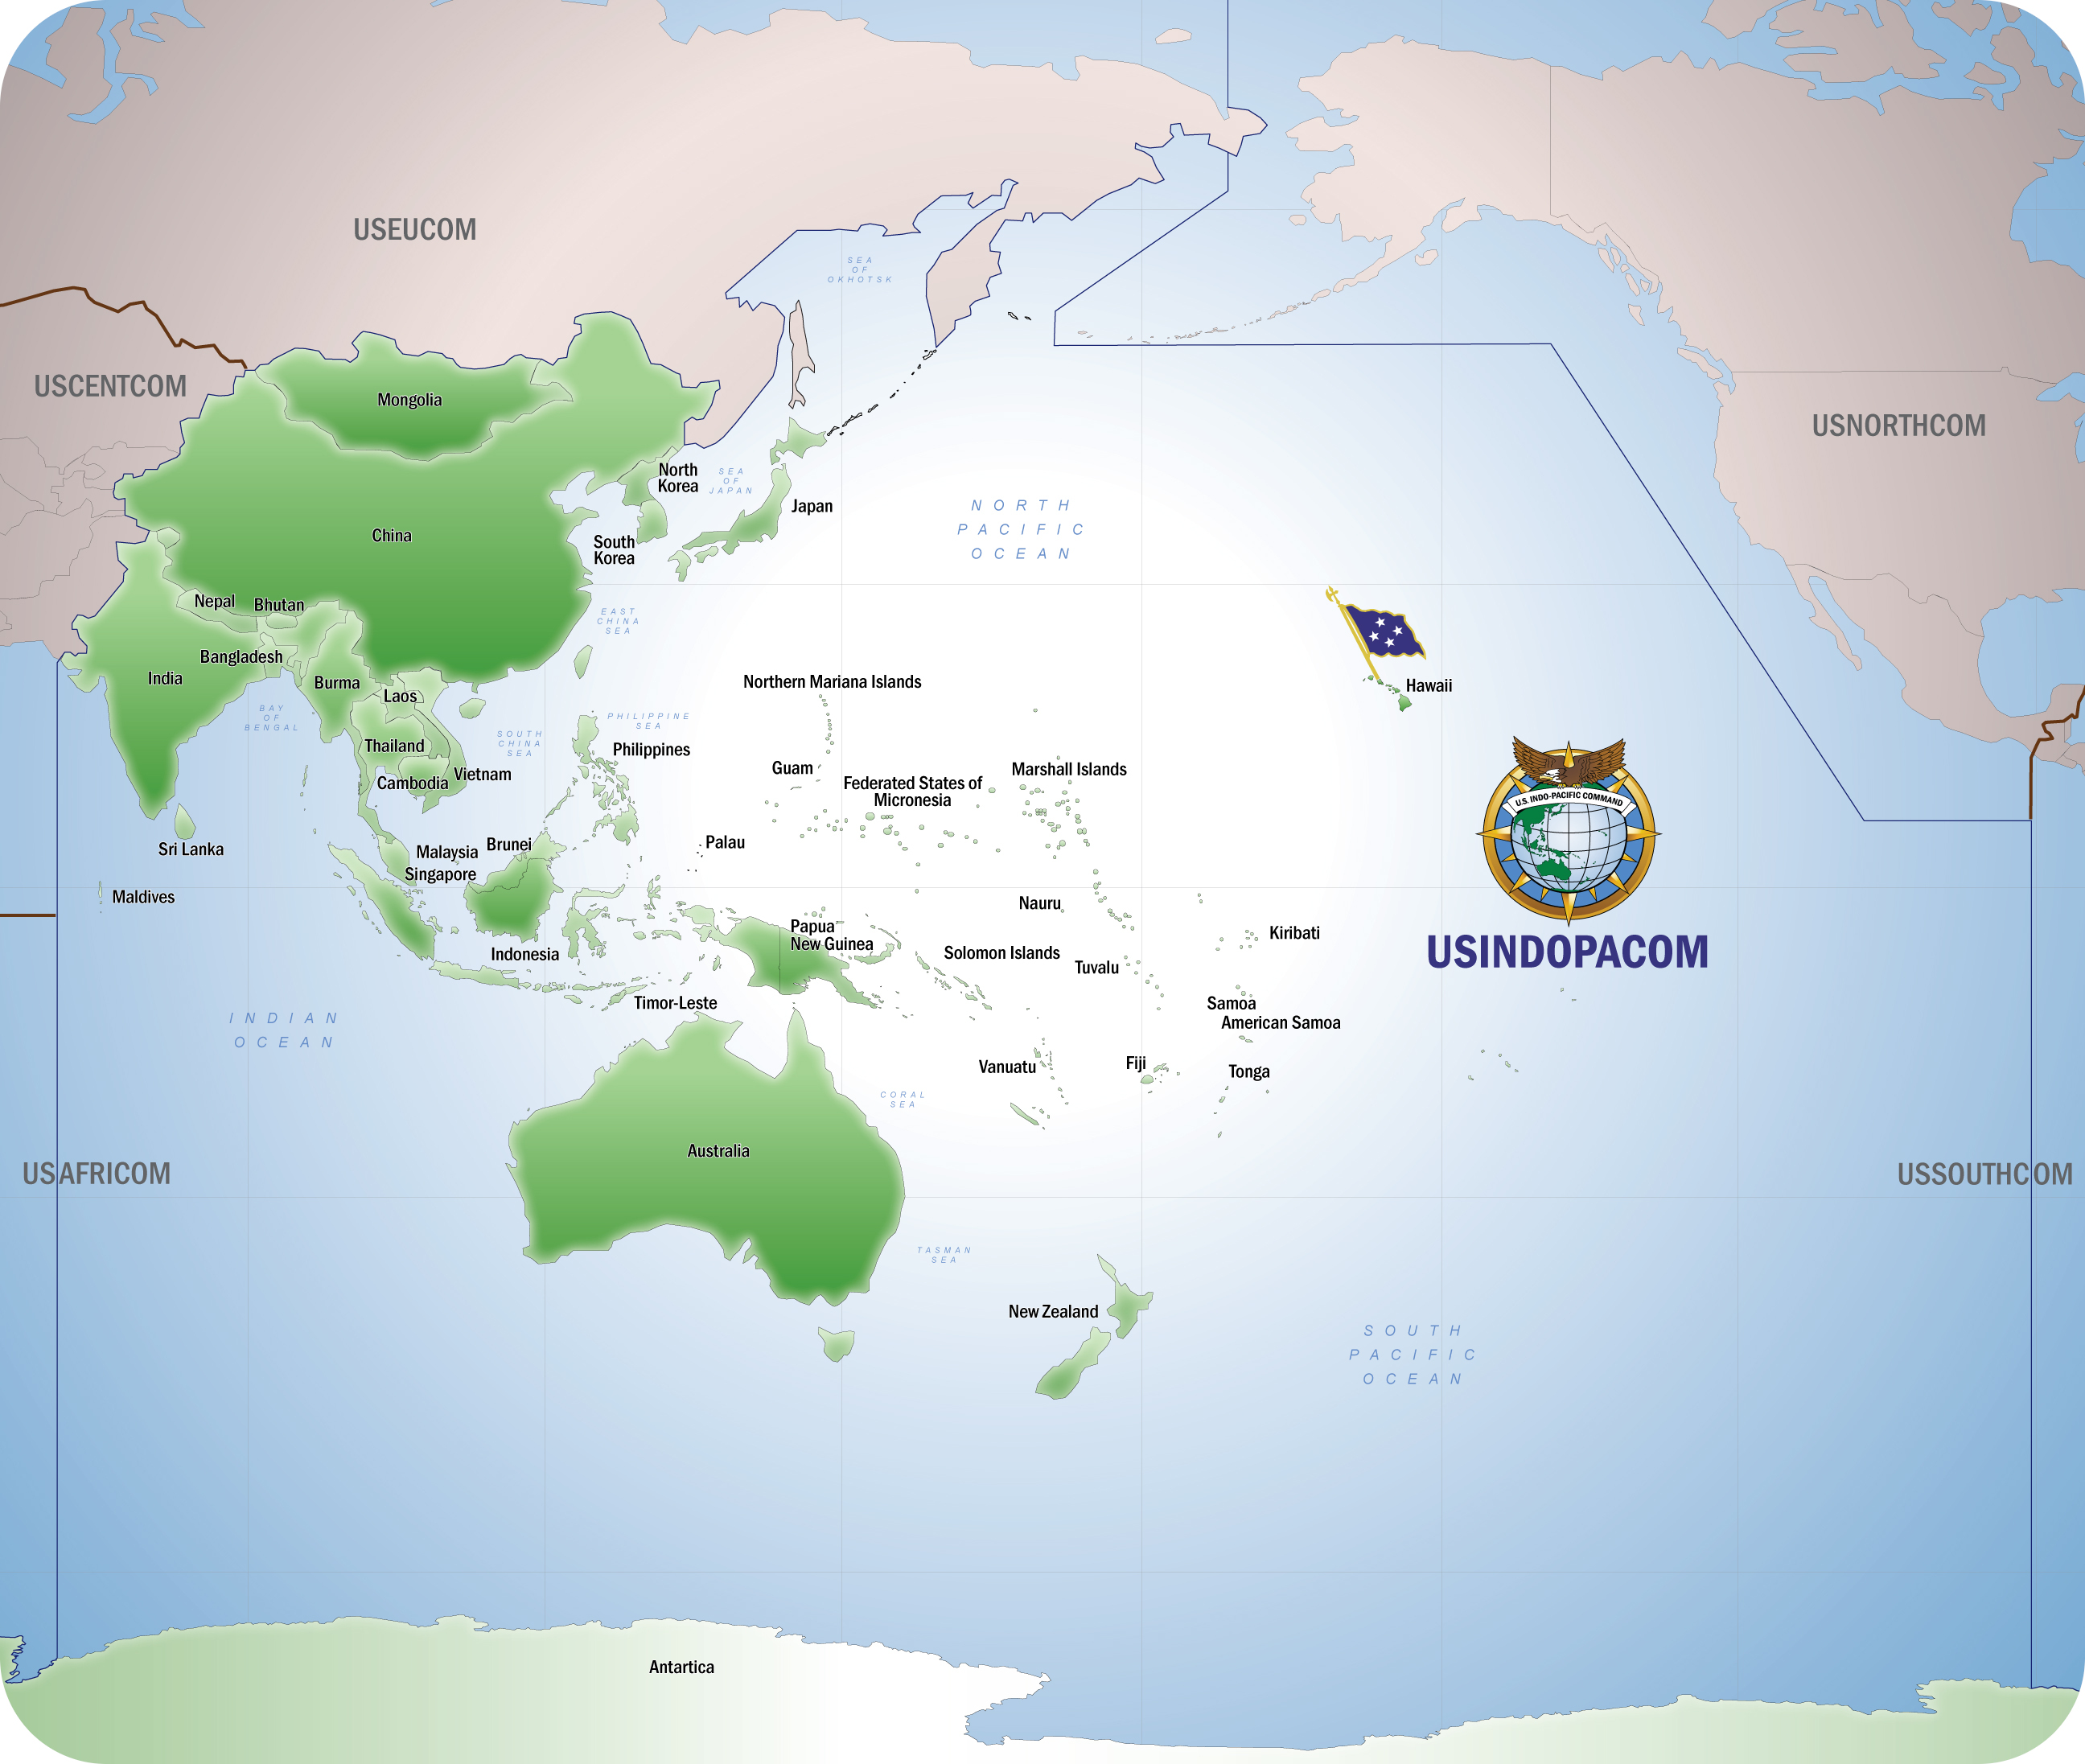
\includegraphics[width=0.65\textwidth]{Images/USINDOPACOM.jpg}
%\caption{Map showing U.S. Military Installations (\footnotesize{\emph{published by PACOM.mil} in 2018})}
%\label{fig:fig2} 
%\end{wrapfigure}
\begin{figure}[h!]
  \centering
  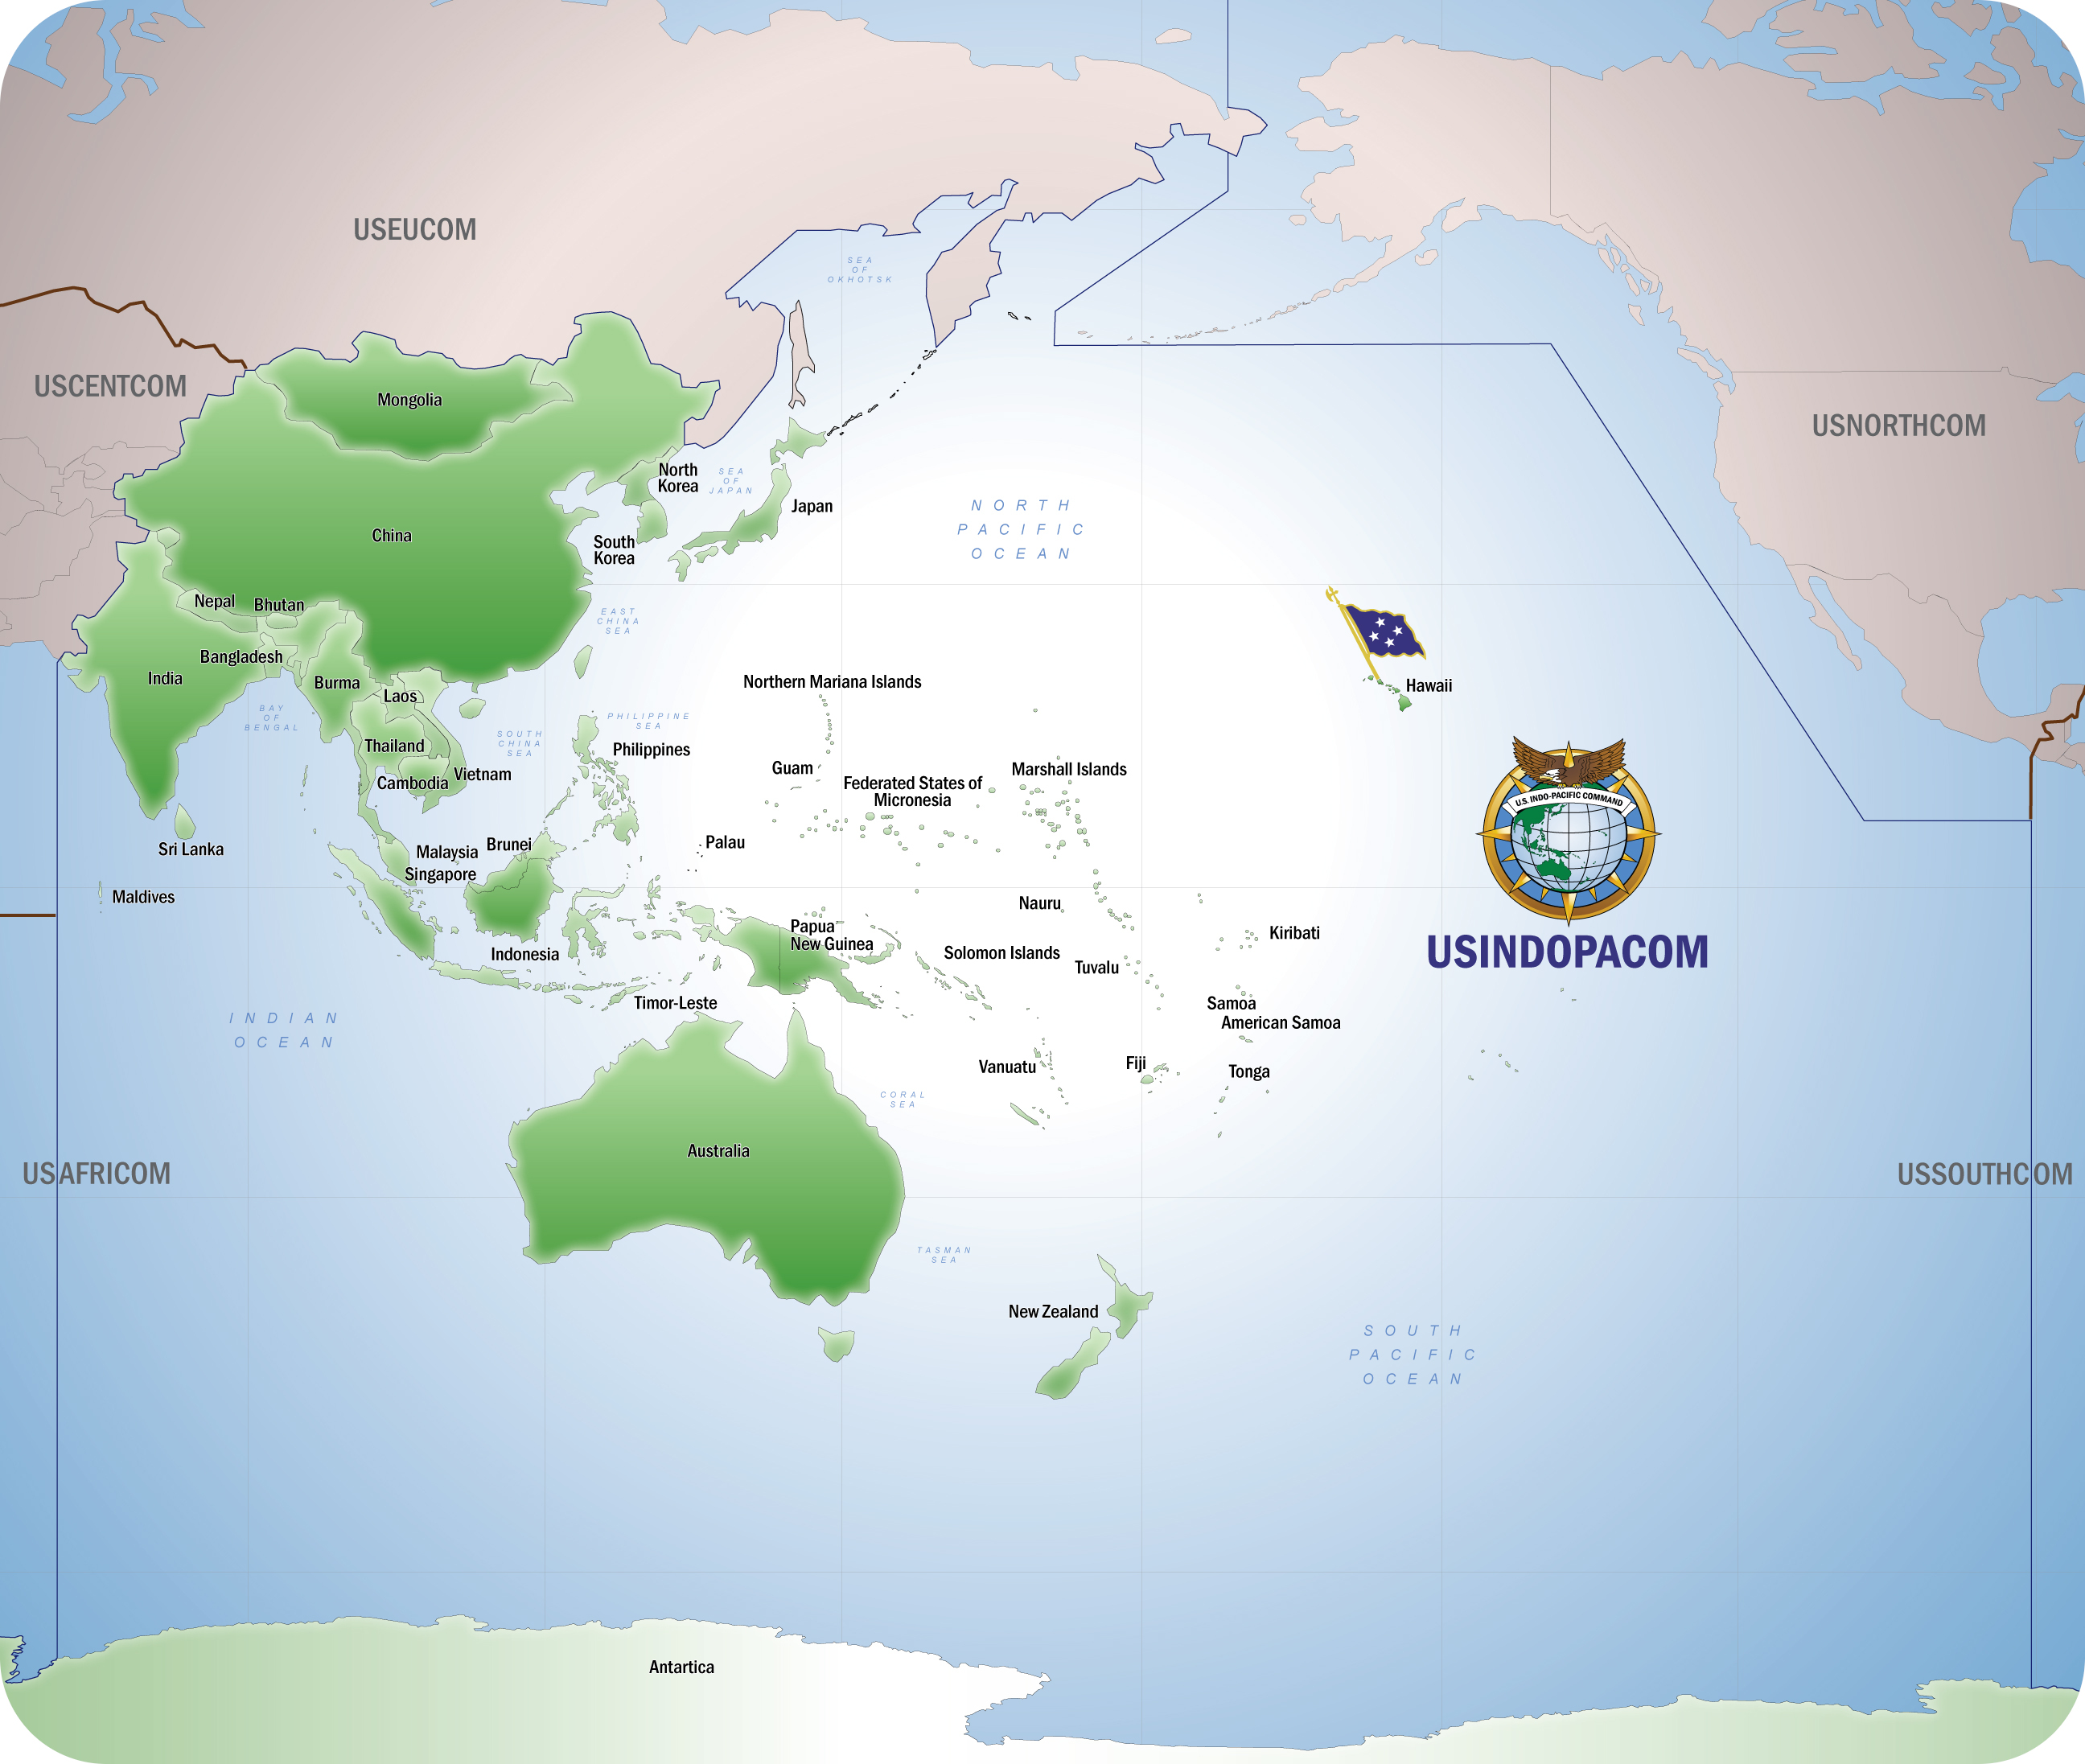
\includegraphics[width=\textwidth]{Images/USINDOPACOM.jpg}
  \caption{Map showing U.S. Military Installations (\footnotesize{\emph{published by PACOM.mil} in 2018})}
  \label{fig:fig2}
\end{figure}


\begin{center}
    \section{\normalsize Jus Ad Bellum}
\end{center}
\begin{center}
\subsection{\normalsize Correlation of Forces}
\end{center}

\paragraph{The Coming War} The People's Liberation Army, comprised of Ground Force, Navy, Air Force, Rocket Force, Strategic Support Force, and the Joint Logistics Support Force is most probably postured for a tellurocratic engagement evident by the miniscule skirmishes along the border with India and distribution of manpower along the Kazakhstan, Mongolian, and Russian borders. The structure and capabilities of the People's Liberation Army are ill prepared for an asymmetric war, as would be the case in Afghanistan, and are “focused largely on waging large-scale land warfare along China’s borders \dots [t]he PLA’s ground, air, and naval forces were sizable but mostly obsolete,” (Department of Defense, 2000). In the Secretary of Defense's annual report to congress entitled “Military and Security Developments Involving the People’s Republic of China 2020”, it is suggested that the Communist Party of China's attempts to modernize and improve the People's Liberation Army have overpassed the United States capabilities concerning shipbuilding, land-based conventional ballistic and cruise missiles, and integrated defense systems. These assertions regarding the status of Chinese military-industrial evolvement indicate the rigor with which the Chinese military-industrial complex approaches their long-term goals; “[the] PLA's objective is to become a “world-class” military by the end of 2049—a goal first announced by General Secretary Xi Jinping in 2017” (Department of Defense, 2020). The difference between The People's Republic of China currently and two decades ago is the modernization of its conscript based statecraft, however according to the aforementioned report to congress, “The PRC's leaders are aware of [major shortcoming and gaps], and their strategy envisions the PLA undergoing almost 30 more years of modernization and reform” (Department of Defense, 2020). What is most important to consider, however, is the undemocratic nature of the Republic of China's statecraft (i.e. conscript induction) and the toll it eventually takes on the uniformed armed services. American ingenuity and resourcefulness is inarguably a product of United States deviationism, those who want to and are able to serve may serve and those who don't qualify either by pretense of the former or latter aren't compelled to. In other words, quality over quantity ensures that, while the People's Liberation Army may boast greater numbers, they are not an analogue to the United States military and their contracted private military companies. The strategic placement of high value United States allies and dependable partner nation-states surrounding the Chinese mainland in southeast Asia (i.e.\ anaconda strategy) provide a commodious theater of operation for the abundant United States military installations in the First Island Chain (The initial archipelago chain from the mainland of China.) and overall Pacific Ocean (refer to \textbf{Figure \ref{fig:fig2}}). Not only do these bilateral partnerships of diplomatic and militaristic origins disbalance any potential conflict in the United States favor, it also puts a tremendous strain on Chinese mainland resources and lines of communication. Historically, a hegemony crumbles from within (i.e. Union of Soviet Socialist Republics, Holy Roman Empire, etc.) and the People's Republic of China is not immune from such an outcome — “the PLA's organizational obstacles were severe enough that, if left unaddressed, they would `inhibit the PLA's maturation into a world-class military force'” (Department of Defense, 2000), two decades later and the narrative still suggests that “[t]he PRC's long-term goal is to create an entirely self-reliant defense-industrial sector—fused with a  strong  civilian  industrial  and  technology  sector—that can meet the PLA's needs for modern military capabilities” (Department of Defense, 2020) notwithstanding the reality that “by 2049 \dots China's strategay can be characterized as a determined pursuit of political and social modernity that includes far-ranging efforts to expand China's national power, perfect its governance systems, and revise the international order” (Department of Defense, 2020). Implying, of course, the perpetual extending of the deadline driven strategy for modernizing the People's Liberation Army. According to the contemporary doctrine on computing correlation of forces and means, “analyses of international affairs consistently assert that a substantial shift in the correlation of forces \dots shifted the main competition from the military arena and towards the economic, political, and ideological spheres” (Deane, 1976), all spheres of influence where the United States is fundamentally advantaegous — Schumpeterian convergence theory of macroeconomics, Marxist-Leninist antideviationism, and the historical shortcomings of communist strongholds all serve as advocates for the conjecture that the Republic of China is behind the United States in both non-militaristic and militaristic respects. If there were to be active military engagements between the United State and the People's Republic of China, they would transpire almost entirely in the Chinese territories along the First Island Chain of the Indo-Pacific Oceans. The United States diplomatic and military missions have been immensely successful at insulating the United States mainland from any potential belligerent blowback. For this reason it can inferred, to the highest degree of confidence, that the United States will remain unprovoked by Chinese aggression and any measure taken to curb said aggression will unequivocally be a retaliatory step toward normalcy. Consequently, the Communist Party of China's ambitiousness to become a “world-class”, tellurocratic, hegemon is as distant a reality as it is a far-fetch deadline. Projections of the year 2049 are merely speculation, and it is completely within the realm of possibilities for the People's Republic of China to degenerate from its contemporary form before the \nth{100} anniversary of its 1949 founding. 
 
\begin{center}
  \section{\normalsize Concluding Remarks}
\end{center}
\paragraph{Contemporary Geopolitical Denouement} Considering the United States and the Republic of China's defense contacts and exchanges in 2019 it becomes obvious that the United States has, does, and most likely will assume a less aggressive, unprovokable position with respect to Chinese aggression in the Indo-Pacific region, “U.S. defense contacts and exchanges conducted in 2019 supported overall U.S. policy and strategy toward China, were focused on reducing risk and preventing misunderstanding in times of crisis, and  were  conducted  in  accordance  with  the  statutory  limitations  of  the  National  Defense Authorization Act for Fiscal Year 2000” (Department of Defense, 2020). The idea that American-Chinese relations could degenerate to an all out conflict is ludicrous, even in the midst of a diplomatically tense trade-war. The realist perspective suggests that the United States and the People's Republic of China are strategic partners and will most probably continue to be so. While the Republic of China has been growing rapidly, it has still not caught up to the United States, if GDP is the preeminent metric, and, outside the scope of particular military-industrial manufacturing and import/export oriented endeavors, does not succeed the United States military-industrial complex. Historically the United States has been involved, politically, economically, and by extension militarily, in thalassocratic/tellurocratic global superpower geopolitical struggles. The current trajectory of United States foreign policy implies that the United States will continue to utilize its position as the chiefest thalassocratic hegemon to “\emph{strangle}” potential tellurocratic competitors. The most important forethought, however, is the prostration of Chinese Foreign Ministry diplomats with respect to negotiating the party line. If not for the Marxist-Leninist nature of the Republic of China's regime of governance, there would be a more constructive approach to maintaining relations with partner nation-states and not just the United States. The existent of the incumbent Chinese regime of governance could mean the demise of the contemporary Chinese mainland pseudo-hegemony if their ideological positions continue to compromises their territorial integrity as was the case with the Soviet Union. The coming war with China will not be a symmetric bilateral struggle but will continue along the trajectory of the ongoing trade-war and, if China replaces the United States as the chiefest foreign power in Afghanistan, will spiral on as the post-World War Two epoch between the United States and Soviet Union. Any action undertaken by the People's Republic of China to realize its 2049 militaristic goals will be met with carefully calculated and deliberate diplomatic and, if necessary, military response, from the more experienced, better suited, and more resourceful United States.

\clearpage

\bibliographystyle{plain}

\begin{center}
  \section{References}
\end{center}

\begin{flushleft}

  Aghion, P., Akcigit, U., & Howitt, P. (2013, February 15). What do we learn from\\\hspace{.5 in}Schumpeterian Growth Theory. \textit{Scholars at Harvard}.\\\hspace{.5 in} \href{https://scholar.harvard.edu/files/aghion/files/what\_do\_we\_learn\_0.pdf}{https://scholar.harvard.edu/files/aghion/files/what\_do\_we\_learn\_0.pdf}\\
  \vspace{5pt}

  Allen, I., & Fitsanakis, J. (n.d.). intelNews.org. \href{https://intelnews.org}{https://intelnews.org}\\
  \vspace{5pt}

  Chan, C. (2020, October 11). Hong Kong bankers are losing their jobs to mainland \\\hspace{.5 in}China rivals. \textit{Bloomberg}. \href{https://www.bloomberg.com/news/articles/2020-10-11/hong-kong-bankers-are-losing-their-jobs-to-mainland-china-rivals}{https://www.bloomberg.com/news/articles/2020-10-\\\hspace{.5 in}11/hong-kong-bankers-are-losing-their-jobs-to-mainland-china-rivals}\\
  \vspace{5pt}

  Deane, M. J. (1976). The Soviet concept of the "Correlation of Forces". \textit{Stanford Research\\\hspace{.5 in} Institute}.\\
  \vspace{5pt}

  Der Führer an das deutsche Volk 22. Juni 1941,” in Philipp Bouhler (ed.), Der \\\hspace{.5 in}großdeutsche Freiheitskampf. Reden Adolf Hitlers, vol. 3 (Munich: Franz Eher,\\\hspace{.5 in} 1942), p. 51-61.\\

  \textit{Geopolitics}. (2002, December 31). \href{https://en.wikipedia.org/wiki/Geopolitics}{https://en.wikipedia.org/wiki/Geopolitics}\\
  \vspace{5pt}

  Hazelbarth, T. (1997). The Chinese media: More autonomous and diverse — within\\\hspace{.5 in} limits. \textit{Central Intelligence Agency}.\\
  \vspace{5pt}

  Hemminki, E., Wu, Z., Cao, G., & Viisainen, K. (2005, August 11). Illegal births and legal\\\hspace{.5 in} abortions — the case of China. PubMed Central (PMC). \\\hspace{.5 in}\href{https://www.ncbi.nlm.nih.gov/pmc/articles/PMC1215519/}{https://www.ncbi.nlm.nih.gov/pmc/articles/PMC1215519/}\\
  \vspace{5pt}

  Kang-chung, N. (2021, June 9). Hong Kong faces brain drain of highly skilled mainland\\\hspace{.5 in} Chinese arrivals: Study. \textit{South China Morning Post}.\\ \hspace{.5 in}\href{https://www.scmp.com/news/hong-kong/society/article/3136690/hong-kong-faces-brain-drain-highly-skilled-mainland-chinese}{https://www.scmp.com/news/hong-kong/society/article/3136690/hong-kong-faces-\\\hspace{.5 in}brain-drain-highly-skilled-mainland-chinese}\\
  \vspace{5pt}

  \newpage

  Lee, K. \textit{Schumpeterian Analysis of Economic Catch-up}.  \\\hspace{.5 in}\href{https://assets.cambridge.org/97811070/42681/frontmatter/9781107042681\_frontmatter.pdf}{https://assets.cambridge.org/97811070/42681/frontmatter/9781107042681\_\\\hspace{.5 in}frontmatter.pdf}\\

  Mackinder, H. J. (1919). \textit{Democratic ideals and reality: A study in the politics of\\\hspace{.5 in} reconstruction}. M.P. London Constable and Company, LTD.\\
  \vspace{5pt}

  Ministry of State Security of the People's Republic of China. \textit{Intelligence Wiki}.\\\hspace{.5 in}  \href{https://intelligence.fandom.com/wiki/Ministry\_of\_State\_Security\_of\_the\_People\%27s\_Republic\_of\_China}{https://intelligence.fandom.com/wiki/Ministry\_of\_State\_Security\_of\_the\_People}\\
  \vspace{5pt}

  Sempa, F. P. (2015, January 21). Is China bidding for the Heartland? \textit{The Diplomat}.\\\hspace{.5 in} \href{https://thediplomat.com/2015/01/is-china-bidding-for-the-heartland/}{https://thediplomat.com/2015/01/is-china-bidding-for-the-heartland/}\\
  \vspace{5pt}

  Spykman, N. J. (1944). \textit{The Geography of Peace}.\\
  \vspace{5pt}

  Wortzel, L. (2013, May 16). Espionage threats at federal laboratories: Balancing scientific\\\hspace{.5 in} cooperation while protecting critical information. \textit{U.S.-China Economic and \\\hspace{.5 in}Security Review Commission}. \\\hspace{.5 in} \href{https://www.uscc.gov/sites/default/files/Wortzel\_Espionage\%20Threat\%20at\%20Federal\%20Laboratories05.16.13.pdf}{https://www.uscc.gov/sites/default/files/Wortzel\_Espionage}\\
  \vspace{5pt}

  \selectlanguage{Russian}Дугин, А. Г. (1999). \textit{Основы Геополитики: Геополитическое Будущее России:\\\hspace{.5 in} Мыслить Пространством}. Arktogeia Tsentr.

\end{flushleft}

\end{document}

